

\tikzset{every picture/.style={line width=0.75pt}} %set default line width to 0.75pt        

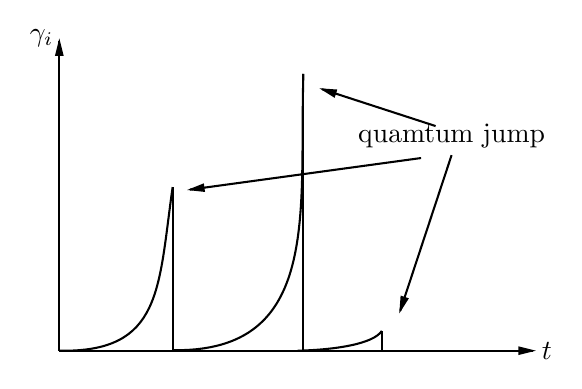
\begin{tikzpicture}[x=0.75pt,y=0.75pt,yscale=-0.7,xscale=0.7]
%uncomment if require: \path (0,300); %set diagram left start at 0, and has height of 300

%Straight Lines [id:da48641940683223894] 
\draw    (127,260) -- (453,260) ;
\draw [shift={(455,260)}, rotate = 180] [fill={rgb, 255:red, 0; green, 0; blue, 0 }  ][line width=0.08]  [draw opacity=0] (12,-3) -- (0,0) -- (12,3) -- cycle    ;
%Straight Lines [id:da418819726200204] 
\draw    (127,260) -- (127,47.06) ;
\draw [shift={(127,45.06)}, rotate = 90] [fill={rgb, 255:red, 0; green, 0; blue, 0 }  ][line width=0.08]  [draw opacity=0] (12,-3) -- (0,0) -- (12,3) -- cycle    ;
%Straight Lines [id:da35056776652524957] 
\draw    (205,147.4) -- (205,259.63) ;
%Straight Lines [id:da15028842415418042] 
\draw    (397,125.4) -- (361.63,232.5) ;
\draw [shift={(361,234.4)}, rotate = 288.28] [fill={rgb, 255:red, 0; green, 0; blue, 0 }  ][line width=0.08]  [draw opacity=0] (12,-3) -- (0,0) -- (12,3) -- cycle    ;
%Curve Lines [id:da6825761392459937] 
\draw    (127,260) .. controls (198,261.4) and (195,217.4) .. (205,147.4) ;
%Curve Lines [id:da6577192720134823] 
\draw    (205,259.63) .. controls (308,261.4) and (292,164.4) .. (295,69.4) ;
%Straight Lines [id:da9977085828752859] 
\draw    (295,69.4) -- (295,260.63) ;
%Curve Lines [id:da10970330232853098] 
\draw    (291,260) .. controls (317,259.4) and (343,255.4) .. (349,246.4) ;
%Straight Lines [id:da19252710913915738] 
\draw    (349,246.4) -- (349,259.4) ;
%Straight Lines [id:da45253685793638243] 
\draw    (376,127.4) -- (216.98,149.13) ;
\draw [shift={(215,149.4)}, rotate = 352.22] [fill={rgb, 255:red, 0; green, 0; blue, 0 }  ][line width=0.08]  [draw opacity=0] (12,-3) -- (0,0) -- (12,3) -- cycle    ;
%Straight Lines [id:da6672435517587316] 
\draw    (386,105.4) -- (307.9,80.01) ;
\draw [shift={(306,79.4)}, rotate = 18] [fill={rgb, 255:red, 0; green, 0; blue, 0 }  ][line width=0.08]  [draw opacity=0] (12,-3) -- (0,0) -- (12,3) -- cycle    ;

% Text Node
\draw (125,45.06) node [anchor=east] [inner sep=0.75pt]    {$\gamma _{i}$};
% Text Node
\draw (457,260) node [anchor=west] [inner sep=0.75pt]    {$t$};
% Text Node
\draw (397,122.4) node [anchor=south] [inner sep=0.75pt]   [align=left] {quamtum jump};


\end{tikzpicture}
